\chapter{HLASM overview}

Assembly languages consist of solely ordinary machine instructions. High-level assemblers generally extend them with features commonly found in high-level programming languages, such as control statements similar to \textit{if, while, for} as well as custom callable macros.

IBM High Level Assembler (HLASM) satisfies this definition and adds other features which will be described in this chapter.

\section{Syntax}

Due to historical reasons, HLASM syntax differs greatly to the syntax of modern programming languages. It mostly uses syntax common to regular assemblers, which has limitations, like line-length limited to 80 characters (as that was the length of a punched card line).

\subsection{Statement}

HLASM program is represented by a sequence of \textit{statements}. A statement consists of four fields. These are:
\begin{itemize}
	\item \textbf{Name field} --- Serves as a place for named constants that are to be used in code. This field is optional, but, when present, it must start at the begin column of a line.
	
	\item \textbf{Operation field} --- The only mandatory field representing the instruction that is executed. Must not begin in the first column, as it would be interpreted as a name field.
	
	\item \textbf{Operands field} --- Field for instruction operands, located immediately after operation field. Individual operands must be separated by a comma, and, depending on the specific instruction, can be either blank, in a form of an apostrophe separated string, or represented by a sequence of characters.
	
	\item \textbf{Remark field} --- Optional, serves as inline commentary. Located either after the operands field, or, in case the operands are omitted, the operation field. 
\end{itemize}

This is an example of a basic statement containing all fields.
\begin{verbatim}
 label   instruction     operands             remarks
.NOMOV       AGO     (&WH).L1,.L2,.L3     SEQUENTIAL BRANCH
\end{verbatim}

\subsection{Continuation}

Individual statements sometimes contain more than 80 characters, which contradicts to line length limitations. Therefore, a special handling called \emph{continuation} is introduced.\todo{Prosim nepouzivejte bold uprostred odstavce nebo v textu, na emphasis a definice je \textbackslash\emph{emph}. Pokud je neco potreba zvyraznit, je to potreba udelat systematictejc, idealne obrazkem.}.

Firstly, let us elaborate more on the topic of line columns. There are four special columns:
\begin{itemize}
	\item \emph{Begin column (default value: 1)}
	
	\item \emph{End column (default value: 71)}
	
	\item \emph{Continuation column (default value: 72)}
	
	\item \emph{Continue column (default value: 16)}
\end{itemize}
They all serve a different purpose.

\textit{Begin column} defines either the start of a statement, or the beginning of the name field.

\textit{End column} determines the end of the statement. Anything written to its right does not count as content of the statement, and is rather used as a place for the line sequence number (see \ref{fig01:line}). 

\textit{Continuation column} is used to indicate that the statement continues on the next line. For proper indication, an arbitrary character other than space must be written in this column. The remainder of the statement must then start on the \textit{continue column}.

Below is an example of an instruction where its last operand exceeded 72.~column of the line.
\begin{verbatim}
  OP1                    REG12,REG07,REG04,REG00,REG01,REG11,Rx
        EG02
\end{verbatim} 

There also exist instructions that support a so called \textit{extended format} of the operands. It allows the presence of a continuation character even when the contents of a line have not reached the continuation column. \todo{reference the figure, do not use [h].}
\begin{verbatim}
  AIF   ('&VAR' FIND '~').A,     REMARK1                      x
        ('&VAR'  EQ  'L').B,     REMARK2                      x
        (T'&VAR  EQ  'U').C      REMARK3 
\end{verbatim} 

\begin{figure}
	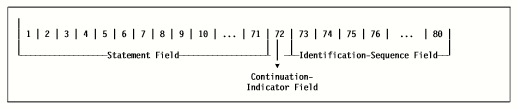
\includegraphics[width=\textwidth]{img/line}
	\caption{Description of line columns (source: HLASM Language Reference https://www-01.ibm.com/servers/resourcelink/\-svc00100.nsf/\-pages/\-zOSV2R3sc264940/\-\$file/\-asmr1023.pdf).}
	\label{fig01:line}
\end{figure}


\section{Assembling}

Having briefly described its syntax, this section prepares the reader to better understand the assembly process hidden behind HLASM. 

We can divide assembling into two interlinked steps --- \emph{conditional assembly} and \emph{ordinary assembly}.

\subsection{Conditional assembly}

The \emph{conditional assembly} process can be compared to a C++ text preprocessor. However, in HLASM, the preprocessing is more complex, so it has obtained the term \textit{code generation}. It works with \emph{variable symbols}, \emph{conditional assembly (CA) instructions} and \emph{macros}. 

\subsubsection{Variable symbols}

Variable symbols serve as points of substitution or information holders. 

When they occur in a statement, they are substituted by their value to create a new statement. For example, in this manner, a user can write a variable symbol in an operation field of a statement and generate any instruction that can be a result of a substitution.

Variable symbols also have notion of their type --- they can be defined either as an integer, a boolean or a string. CA instructions gather this information for different sorts of conditional branching.

\subsubsection{CA instructions}

The major difference to other instructions is that they are not assembled into object code. Rather, they select which instructions will be processed by assembler next.

One subset of CA instructions operates on variable symbols. With them, the user can define variable symbols locally or globally, assign or update their values.

Other subset is capable of conditional and unconditional branching. HLASM provides a variety of built-in binary or unary operations on variable symbols, which can create complex conditional expressions. This is important in HLASM, as the user can alter flow of instructions that will be assembled into executable program.

\subsubsection{Macros}

A \emph{macro} is a structure consisting of a \emph{name}, \emph{input parameters} and a \emph{body}, which is a sequence of statements. When a macro is called in a HLASM program, each statement in its body is executed. Both nested and recursive calls of macros are allowed. Macro body can even contain a sequence of instructions generating another macro definition.

With the help of variable symbols, HLASM macros have the power to create custom, task specific macros.

\subsection{Ordinary assembly}

Ordinary assembly is a term for assembly other that conditional. It includes assembly of both machine and assembler instructions. 

\emph{Machine instructions} and their operands are translated to a sequence of bytes and written to the executable program. In contrast to basic assemblers, HLASM allows expressions to be passed as operands of these instructions. These expressions are capable of address arithmetics, and can also contain defined constants.

\emph{Assembler instructions}, on the other hand, are used to alter the behavior of the assembler. Therefore, they are not assembled into the executable program.

\subsubsection{Assembler instructions}

A few specific instructions exist that alter assembler's behavior. Let us name a few of them:
\begin{itemize}
	\item \textbf{ICTL} --- Changes values of the previously described line columns (i.e. begin column may begin at column 2 etc.).
	
	\item \textbf{DC} --- Reserves space in object code for data described in operands field and assembles them in place (i.e. assembles float, double, character array, address etc. ).
	
	\item \textbf{EQU} --- Defines named constant with an integer or a relative address value. These constants can be accessed by \textit{conditional assembly}, hence alter it in custom manner.
	
	\item \textbf{COPY} --- Copies a whole file found in \textit{copy member library}\footnote{Path to library is passed to assembler before the start of assembly} and pastes it in place of the instruction.
	
	\item \textbf{CSECT} --- Creates an executable control section. Serves as the beginning of a machine instruction sequence and as the start of relative addressing.
\end{itemize}

Below is an example of a simple HLASM program with the description of its statements:

\begin{verbatim}
         name        operation   operands
         
[01]                 MACRO                   
[02]     &NAME       GEN_LABEL
[03]     &NAME       EQU         *
[04]                 MEND
[05]             
[06]                 COPY        REGS
[07]             
[08]     TEST        CSECT
[09]     &VAR        SETA        L'DOUBLE
[10]                 AIF         (&VAR EQ 4).END
[11]     LBL1        GEN_LABEL
[12]                 LR          3,2
[13]                 L           8
[14]     LBL2        GEN_LABEL
[15]     LEN         EQU         LBL2-LBL1
[16]                 DC          (LEN)C'HELLO'
[17]     DOUBLE      DC          D'-3.729'
[18]     .END        ANOP
[19]                 END
\end{verbatim} 

In lines \verb|01-04|, we see a \emph{macro definition}. It is defined with a name \verb|GEN_LABEL|, variable \verb|NAME| and contains one instruction in its body, which assigns the current address to the label in \verb|NAME|.

In line \verb|06|, the \emph{copy instruction} is used, which includes the contents of the \verb|REGS| file.

Line \verb|08| establishes a start of an executable section \verb|TEST|. 

In line \verb|09|, an integer value is assigned to a variable symbol \verb|VAR|. The value is the length attribute of previously non-defined constant \verb|DOUBLE|. The assembler looks for the definition of the constant to properly evaluate the conditional assembly expression. In the next line, there is CA branching instruction \verb|AIF|. If value of \verb|VAR| equals to 4, next lines are skipped and assembling continues on line \verb|18|, where branching symbol \verb|END| is located.  

Lines \verb|12-13| show examples of machine instructions that are directly assembled into object code. Lines \verb|11,14| contain examples of macro call.

In line \verb|15|, the constant \verb|LEN| is assigned the difference of two addresses. This value is next used to generate character data.

Instruction \verb|DC| in line \verb|17| creates value of type double and assigns its address to constant \verb|DOUBLE|. This constant also holds information about length, type and other attributes of the data.  

\verb|ANOP| is an empty assembler action and line \verb|19| ends the assembling of the program. 

\vspace{5mm}